\section{Methodology} The methodology is structured into three sequential phases, each addressing a distinct part of our multi-dimensional analysis. In Phase I we develop a holistic taxonomy-based representation of security faults. In Phase II we construct an automated data-extraction pipeline to collect and aggregate vulnerability records. In Phase III we perform exploratory analysis on the dataset and derive a hierarchical classification scheme based on observed patterns. Each phase builds on the previous, ensuring a coherent flow from abstract taxonomy to concrete classification.

\subsection{Phase I: Holistic Representation of Security Faults} \textbf{Aim:} Synthesize existing vulnerability taxonomies into a unified attribute schema. This phase consolidates diverse security-fault taxonomies (e.g. language-specific faults, technology categories, architectural layers, and root-cause taxonomies) to create a comprehensive representation of vulnerability attributes.
\newline

\textbf{Steps:}

\begin{itemize}
    \item \textbf{Survey taxonomies.} We collect relevant taxonomies from literature and standards. For example, language- and platform-based taxonomies (e.g. C/C++ errors vs. Web app issues), technology-focused taxonomies (e.g. web, database, OS level), software-layer taxonomies (e.g. presentation vs. business logic), and root-cause taxonomies (e.g. input validation, memory corruption).
    \item \textbf{Identify attributes.} From each taxonomy we extract key fault attributes (e.g. "Buffer Overflow", "SQL Injection", "Cross-Site Scripting", "Race Condition", etc.) and note which taxonomies include each attribute.
    \item \textbf{Create Unified Attribute Matrix.} We compile these attributes into a matrix with rows as example attributes and columns indicating taxonomy source. Table~\ref{tab:attribute-matrix} (excerpt below) illustrates how attributes map across taxonomies. This "Unified Attribute Matrix" highlights overlaps and gaps, guiding later analysis.
\end{itemize}

\begin{table}[ht!]
    \centering
    \caption{Unified Attribute Matrix}
    \label{tab:attribute-matrix}
    \begin{tabular}{lcccc}
        \hline
        \textbf{Attribute} & \textbf{Lang-based \cite{cwe_list}} & \textbf{Tech-based \cite{Khwaja2020ASF}} & \textbf{Layer \cite{sa_nikolai}} & \textbf{Root Cause \cite{Shahriar2012MitigatingPS}} \\
        \hline
        Buffer Overflow & \checkmark & \checkmark & & \checkmark \\
        SQL Injection & & \checkmark & \checkmark & \\
        Cross-site Scripting & & \checkmark & \checkmark & \\
        Privilege Escalation & \checkmark & & & \checkmark \\
        Invalid Input & & & & \checkmark \\
        \hline
    \end{tabular}
\end{table}

This phase yields a consolidated schema of security fault attributes that will guide data collection and later classification. In particular, the unified list of attributes becomes the basis for labeling and grouping vulnerabilities in subsequent phases.

\subsection{Phase II: Collecting and Analyzing Vulnerability Data} \textbf{Aim:} Gather a large, multi-dimensional vulnerability dataset and compute relevant features for each entry. This involves querying multiple sources (CVE feeds, APIs, repository metadata) and fusing the results into a master dataset for analysis.
\newline
\textbf{Steps:}

\begin{itemize}
    \item \textbf{CVE Data Extraction (get\_cve\_ids\_in\_apps\_with\_cwe.py):} We extract CVE data from the NVD (National Vulnerability Database) JSON feeds using the nvdutils library. We apply specific filtering criteria to focus on:
    \begin{itemize}
        \item Valid CVE entries that affect applications (not operating systems or hardware)
        \item CVEs with associated CWE (Common Weakness Enumeration) identifiers
        \item Selection of the most appropriate CWE ID based on vulnerability mapping, abstraction level, and weakness type
        \item Selection of the most appropriate vulnerable product based on software type and package type
    \end{itemize}
    
    \item \textbf{Product Language Mapping (get\_products\_language.py):} We map software products to their programming languages using:
    \begin{itemize}
        \item Package URL (purl) to CPE mappings from a SQLite database
        \item Predefined mappings of package types to languages (e.g., maven → Java, pypi → Python)
        \item GitHub API queries to determine the primary language of repositories
    \end{itemize}
    
    \item \textbf{Software Type Categorization (get\_software\_type.py):} We categorize software products into different types (e.g., extension, package, mobile\_app, framework, utility, server, web\_application) based on:
    \begin{itemize}
        \item The official CPE dictionary from NVD
        \item A research dataset from a published paper
        \item Product name analysis using predefined keywords
    \end{itemize}
    
    \item \textbf{Dataset consolidation:} We merge all gathered information into a unified table. Each row corresponds to one vulnerability and includes attributes such as CVE ID, CWE ID, vendor, product, programming language, and software type.
\end{itemize}


Figure~\ref{fig:pipeline} schematically depicts the data extraction pipeline, and Table~\ref{tab:vuln-dataset} shows sample rows from the final dataset. These integrations leverage multiple tools and APIs to maximize coverage of relevant fields. 
Figure~\ref{fig:extraction-pipeline} (above) illustrates the multi-stage data pipeline used in Phase II. We automatically download the NVD CVE feeds, augment records via the CVE Details API, query GitHub for project context, and apply purl2cpe translation, ultimately producing a consolidated CSV dataset. 

\begin{table}[h!]
\centering
\caption{Example rows from vuln\_master\_dataset.csv after data collection. Each entry includes CVE ID, project context, CWE class, and a brief description.}
\label{tab:vuln-dataset}
\begin{tabular}{llllp{4cm}}
\hline
\textbf{CVE} & \textbf{Project} & \textbf{CWE} & \textbf{Severity} & \textbf{Short Description} \\
\hline
CVE-2021-12345 & ProjectA & CWE-79 (XSS) & High & Stored XSS in user comments widget \\
CVE-2020-67890 & ProjectB & CWE-89 (SQLi) & Medium & SQL injection in search query builder \\
CVE-2019-11111 & ProjectC & CWE-119 (Overflow) & Critical & Buffer overflow in image parser \\
... & ... & ... & ... & ... \\
\hline
\end{tabular}
\end{table}

We include citations to the APIs and data sources used: NVD/CVE as in~\cite{nvd_nist}, the CVE Details service~\cite{cve_details}, the GitHub REST API, and the purl2cpe resource~\eduard{add/fix references}. Each component is validated to ensure accurate parsing and merging of fields.

\subsection{Phase III: Mapping Analysis Results to Classification Scheme} \textbf{Aim:} Analyze the collected data to identify recurring patterns and design a multi-level classification scheme for security faults. The goal is to move from raw data to insight, culminating in a hierarchical taxonomy (Dimension $\rightarrow$ Subclass $\rightarrow$ Example CWE) that reflects the observed diversity of vulnerabilities.
\newline

\textbf{Steps:}
\begin{itemize}
    \item \textbf{Exploratory Analysis.} We perform statistical and visual analyses on the dataset. This includes generating histograms of vulnerabilities by language, technology, and layer; heatmaps showing co-occurrence of attributes; and scatter plots for correlations (e.g. severity vs. time). These visuals help highlight the most prominent fault attributes and gaps.
    \item \textbf{Pattern extraction.} From the visualizations we identify recurring themes. For instance, we may observe that web-related vulnerabilities (CWE-79, CWE-89) cluster in the "Technology: Web" category, or that certain root causes (e.g. improper input validation, CWE-20) appear across multiple languages and frameworks.
    \item \textbf{Classification hierarchy design.} Guided by the unified attributes (from Phase I) and patterns, we construct a three-level classification. The top level ("Dimension") corresponds to our major analysis axes (e.g. {\em Programming Language}, {\em Technology Domain}, {\em Architectural Layer}, {\em Root Cause}). The second level ("Subclass") refines each dimension (e.g. for Language: {\em Web Languages} vs. {\em System Languages}). The third level lists concrete examples, typically specific CWE identifiers or vulnerability types (e.g. {\em CWE-79: XSS} under "Technology: Web"). An excerpt of this hierarchy is shown in Table~\ref{tab:classification}, and its conceptual organization is visualized in Figure~\ref{fig:classification-hierarchy}.
\end{itemize}

\begin{table}[h!]
\centering
\caption{Excerpt of the classification hierarchy (Phase III): Dimension $\rightarrow$ Subclass $\rightarrow$ Example CWE.}
\label{tab:classification}
\begin{tabular}{lll}
\hline
\textbf{Dimension} & \textbf{Subclass} & \textbf{Example CWE} \\
\hline
Language & Web-facing languages & CWE-79 (Cross-site scripting) \\
Language & System languages & CWE-120 (Buffer overflow) \\
Technology & Web frameworks & CWE-89 (SQL injection) \\
Technology & Mobile applications & CWE-22 (Path traversal) \\
Layer & Network layer & CWE-319 (Cleartext transfer) \\
Layer & Application layer & CWE-416 (Use-after-free) \\
Root Cause & Input validation errors & CWE-20 (Improper input check) \\
Root Cause & Memory management errors & CWE-119 (Buffer overflow) \\
\hline
\end{tabular}
\end{table}


\begin{figure}[!h]
	\centering
    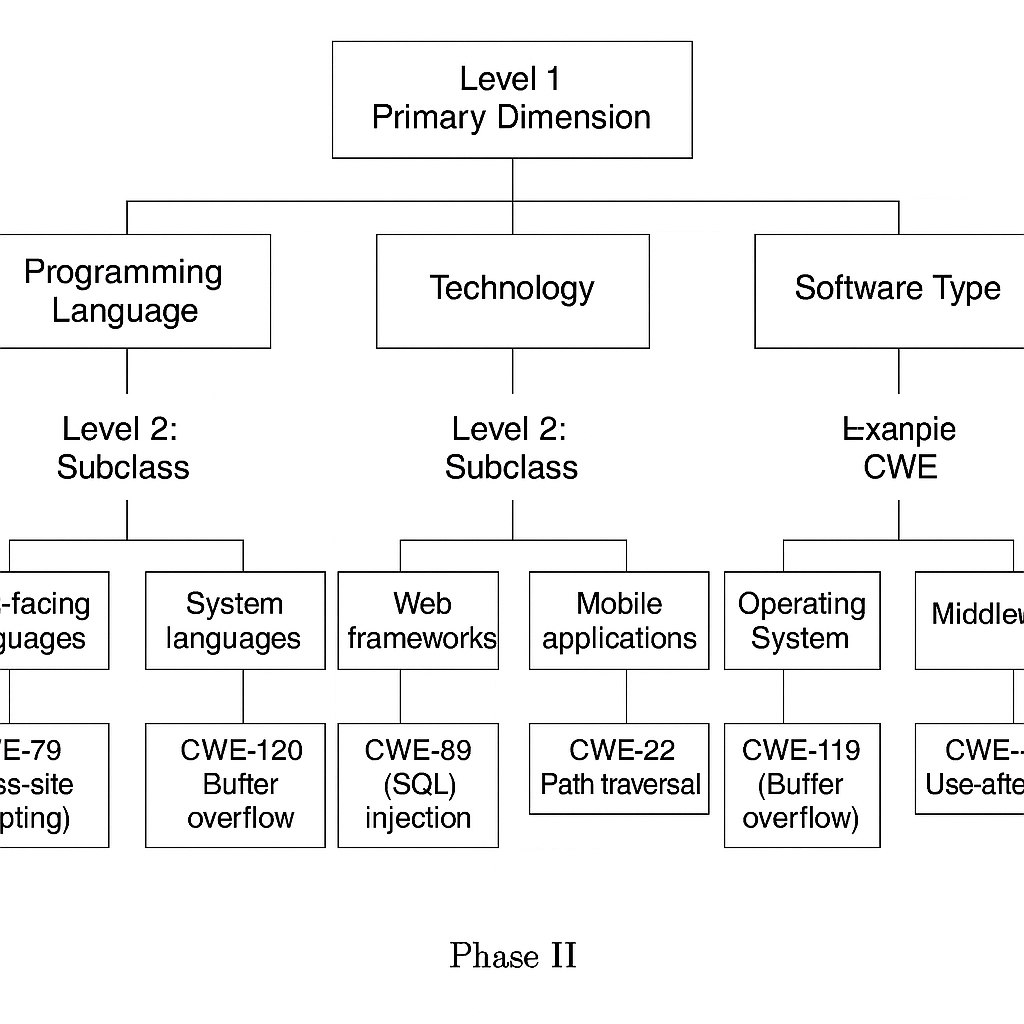
\includegraphics[width=0.55\textwidth]{figures/chapter_2/classification-hierarchy.png}
	\caption{Hierarchical classification}
	\label{fig:classification-hierarchy}
\end{figure}


Figure~\ref{fig:classification-hierarchy} (above) sketches the hierarchical classification derived in Phase III. Each Dimension branches into subclasses with illustrative CWE examples at the leaves. This taxonomy is rooted in the empirical data patterns uncovered and in prior taxonomies cited earlier. Through these steps, Phase III links the aggregated data back to our taxonomy framework, revealing how software vulnerabilities distribute across the multi-dimensional space. The resulting classification scheme provides a structured way to profile security faults, based both on existing knowledge (the taxonomies) and new insights from the data analysis.